\section{Методика}

	Суть работы заключается в анализе данных наблюдений рентгеновских пульсаров и кандидатов в черные дыры с космических аппаратов, дальнейшее определение параметров таких особенностей компактных объектов, как квазипериодические осцилляции и их эволюция со временем.

	%Методика состоит в поиске значимых гармоник в спектрах мощности временных историй счета гамма-излучения космического гамма-излучения и сопоставление их с известными источниками данные к которым приведены, например в статье Ларса Бильдстена <<Observation of Accreting Pulsars>> (в ней представлены характеристики аккрецирующих пульсаров на момент 1997 года). Для MAXI J1820+070 предполагается анализ квазипериодических осцилляции, регистрируемых как широкая линия в спектре мощности.
	
	Данные наблюдения взяты с трех приборов: Konus-Wind, INTEGRAL/ISGRI и Swift/BAT. Они представляют собой несколько массивов чисел, означающих количество считанных фотонов за единицу времени на разных энергетических диапазонах.
	
	Для анализа квазипериодических осцилляций используется спектр мощности сигнала, полученный из временных историй скоростей счёта гамма-квантов преобразованием Фурье, о котором написано ниже.
	
	При анализе кандидата в черную дыру временная история разбивается на равные части определенной длительности (в нашем случае --- 1 день). Для каждого участка строится его спектр мощности, который затем аппроксимируется степенной функцией вида $f^{-1}$ и распределением Гаусса при помощи так называемого метода наибольшего правдоподобия. В результате выполнения программы находится частота квазипериодических колебаний.
	
	Полученные значения частот далее сравниваются с характерными частотами осцилляций черных дыр из статьи C. E. Мотта \cite{black_hole} для определения состояния объекта.
	
\section{Математические методы}
	
	\subsection{Cпектр мощности сигнала}
		
%		Большую часть процессов переменности яркости астрономических объектов трудно описать, поскольку процесс является стохастическим. Переменность является <<суммой>> отдельно взятых процессов, количество которых может быть довольно велико. (можно представить аналогию с газом, где малые колебания поршня являются суммарным действием молекул газа, которые двигаются по определенным законам, но молукул настолько много, что процесс нельзя описать, отдельно учитывая каждую молекулу).
		
%		Поскольку в стохастических процессах сигнал невозможно учесть все детали кривой блеска, то модель стохастического процесса должна описывать общие свойства сигнала. Чтобы иметь возможность строить такие модели и сравнивать их с наблюдениями, общие свойства сигнала не должны зависеть от времени, т.е. стохастический процесс, формирующий сигнал, должен быть так же и стационарным.

%		Ряды Фурье или преобразование Фурье позволяет выделить определяющие свойства сигнала и тем самым провести анализ временной переменности яркости астрономических объектов.
		
		Преобразованием Фурье функции $f(x)$ называется функция $\hat{f}(\omega)$:
		
		\begin{equation}
			\hat{f}(\omega) = \int\limits^{+\infty}_{-\infty} f(x) e^{-2 \pi i x \omega} \, \mathrm{d} x
		\end{equation}		 
		
		Поскольку в реальности сигнал является ограниченным во времени, а также дискретным (т.е. сигнал является набором точек), то вместо преобразования Фурье используется дискретное преобразование Фурье, которое записывается в таком виде:
		
		\begin{equation}
			X (k) = \sum^{N - 1}_{n = 0} x (n) e^{-\frac{2 \pi i}{N} k n}, \text{где}
		\end{equation}
		
		$x_n$ --- изначальный набор данных, $N$ ---	количество точек, в изначальном наборе данных, а $X_k$ --- набор данных, полученный после преобразования.
		
		Одним из свойств преобразования Фурье (и соответственно дискретного преобразования) является теорема Парсеваля, которая записывается как:
		 
		\begin{equation}
			\sum\limits^{N - 1}_{n = 0} |x (n)|^2 \, = \frac{1}{N} \sum\limits^{N - 1}_{k = 0} |X (k) |^2
		\end{equation}
		
		Свойство физически означает, что при преобразовании Фурье энергия сигнала (условный квадрат амплитуды) сохраняется.
		
		~
		
		Если нормировать мощность сигнала $P_j$ (изначальный квадрат амплитуды), как:
		
		\begin{equation}
			P_j = \frac{2 | X_j |^2 }{N_{\gamma}}, \text{где}
		\end{equation}
		
		$N_{\gamma}$ --- суммарное количество фотонов в приходящем сигнале, то можно доказать, что, считая процесс пуассоновским (т.е. детектор идеальный), полученная величина подчиняется 
		%Такая нормировка упрощает нахождение значимых гармоник, поскольку тогда можно доказать, что для идеального пуассоновского процесса (т.е. наблюдения гораздо больше единичного времени счета, а также ) мощность сигнала 
		распределению $\chi^2$ с двумя степенями свободы. $\chi^2_2$ распределение имеет такой вид: $p( x ) d x = \exp( -x / 2 ) / 2 d x$. Для данного распределения верно, что средняя мощность сигнала $\left\langle P_j \right\rangle = 2$, а вероятность превысить данное значение x: $P( > x) = \exp( -x / 2)$. Так можно находить значимые гармоники с определенной вероятностью, например $3\sigma$ или $5\sigma$ (если мощность сигнала на данной гармонике с определенной вероятностью выше среднего). На рис. \ref{img:sp} представлен спектр мощности тестового сигнала с одной гармоникой.
		
	\begin{figure}[h!]
		\centering
		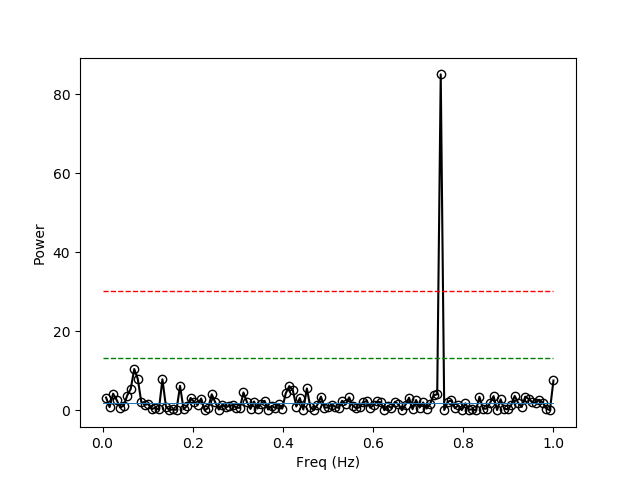
\includegraphics[width = 0.65\linewidth]{pictures/PDS.png}
		\caption{Спектр мощности тестового сигнала с частотой 0{,}75 Гц. Синим обозначено среднее значение шума. Красным обозначен сигнал с вероятностью $5 \sigma$, а зеленый с вероятностью $3 \sigma$}
		\label{img:sp}
	\end{figure}

		 
	%	\cite{m.vanderklis1988}
	% написать про преобразование Фурье и попытаться провести с чем-то аналогию\cite{vikhlinin_dissertation}
	
	\newpage
	
	\subsection{Метод наибольшего правдоподобия}
	
		Наиболее часто встречающийся метод аппроксимации спектра мощности различными моделями --- метод наибольшего правдоподобия. 
		
		Он состоит в максимизации так называемой функции правдоподобия, которая является произведением вероятностей при модельном значении $y_i$ иметь экспериментальное значение $x_i$: $\mathrm{L} = \prod p ( x_i | y_i )$. 
		
		Поскольку логарифм --- монотонная, возрастающая функция, то обычно от функции правдоподобия берут логарифм, поскольку сумма значений считается проще, чем их произведение. Также чаще функцию аппроксимации минимизируют, поэтому от всего выражения берут минус и в итоге получается, что функция максимального правдоподобия записывается таким образом: 
		
		$$ L = - \ln \prod p ( x_i | y_i ) = - \sum \ln ( p ( x_i | y_i ) )$$
		
		В данном случае плотность вероятности $p ( I_j | S_j )$ при модельном значении мощности $S_j$ иметь экспериментальное значение $I_j$ равна:
		
		\begin{equation}
			p ( I_j | S_j ) = \frac{1}{S_j} \exp ( - I_j / S_j)
		\end{equation}
		
		Тогда для нее функция правдоподобия записывается таким образом:
		
		\begin{equation}
			L = - 2 \ln \prod \frac{1}{S_j} \exp ( - I_j / S_j) = 2 \sum \left( I_j / S_j + \ln ( S_j ) \right)
		\end{equation}

\section{Инструменты}
	
	Конус --- гамма-спектрометр, установленный на космический аппарат \textit{GGS-Wind}. Конус-Винд состоит из двух одинаковых NaI(Tl) сцинтилляционных гамма-спектрометров (S1 и S2), расположенных на противоположных сторонах космического аппарата, что обеспечивает обзор всей небесной сферы. Каждый детектор состоит из кристалла NaI(Tl), который  просматривается фотоэлектронным умножителем (ФЭУ) через свинцовое стекло, нужное для снижения фонового излучения от космического аппарата. Попадая в детектор, гамма-квант передаёт часть или всю свою энергию
веществу сцинтиллятора, которая преобразуется в световую вспышку, регистрируемую ФЭУ. Заряд, собранный с анода ФЭУ, преобразуется в импульс напряжения, который усиливается и формируется для получения максимального отношения сигнал-шум, после чего амплитуда импульса измеряется аналого-цифровым преобразователем (АЦП). Схематический вид прибора и аппарата представлен на рис. \ref{img:kw1} \cite{Svinkin_thesis}. Прибором ведется запись в 4 энергитических каналах: G1 (13 -- 50 кэВ), G2 (50 -- 200 кэВ), G3 (200 -- 760 кэВ) и Z (>10 МэВ) \cite{aptekarr.l.1993}.

	\begin{figure}[h!]
		\centering
		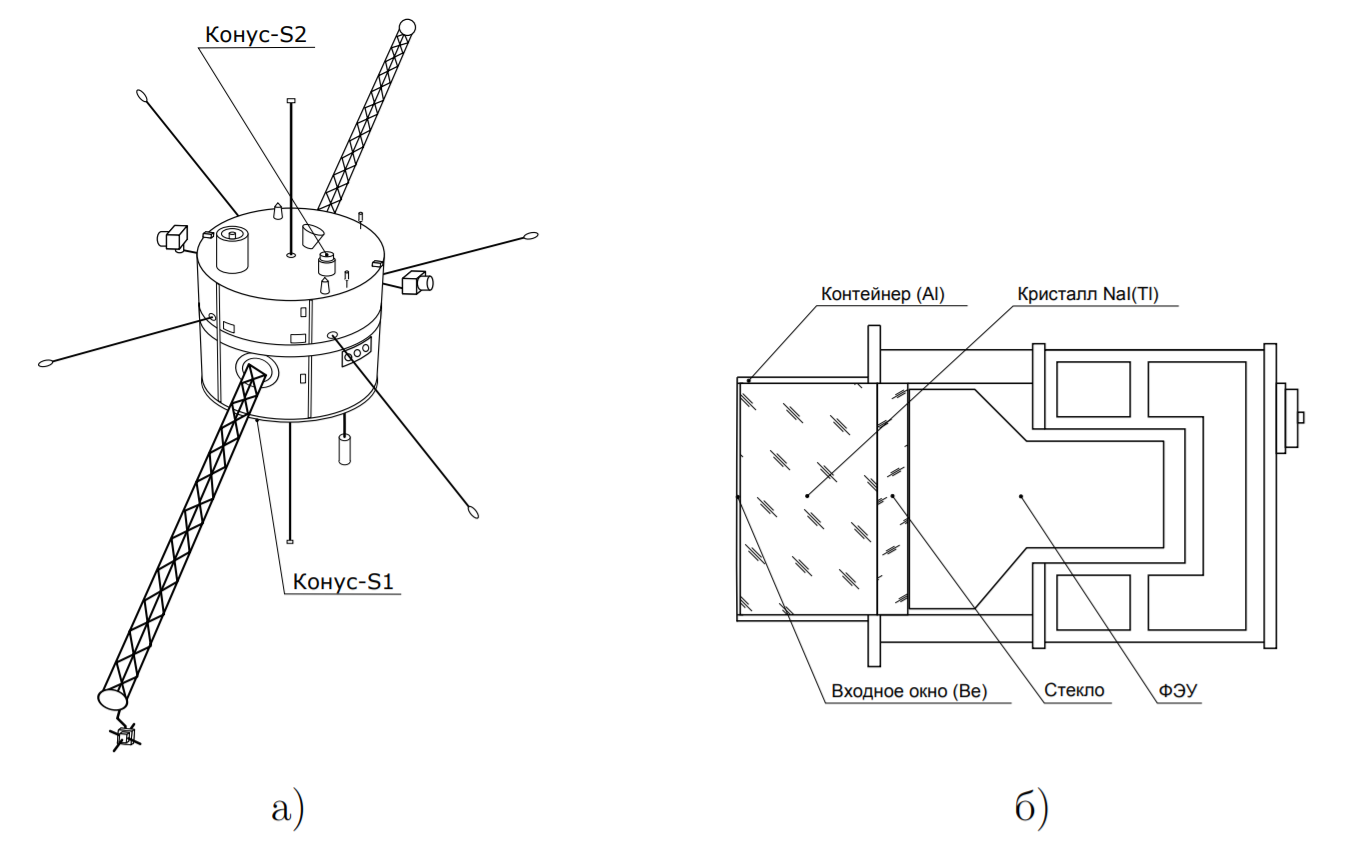
\includegraphics[width = 0.65\linewidth]{pictures/Konus-Wind.png}
		\caption{Устройство (а) спутника \textit{GGS-Wind} и (б) самого прибора}
		\label{img:kw1}
	\end{figure}
	
	BAT --- один из инструментов орбитальной обсерватории SWIFT, представляющий из себя телескоп с кодирующей маской. Кодирующая апертура является одним из способов построения изображения источника в жестком рентгеновском и мягком гамма диапазоне без использования системы линз и зеркал. Метод широко применяется в гамма- и рентген-астрономии, в том числе и в INTEGRAL/ISGRI. Линзы и зеркала в астрономии высоких энергий не используются, поскольку при попадании на линзу рентгеновские и гамма-кванты почти не преломляются и либо проходят насквозь стекло, либо поглощаются материалом. Сигнал регистрирует массив CdZnTe-детекторов, половина которых закрывается маской. В отличие от Konus-Wind, его поле зрения меньше и равняется $1.4$ стерадиана. На рис. \ref{img:bat1} можно увидеть схематическое представление прибора.
	 
	 CdZnTe-детекторы также, как и CdZn являются полупроводниковыми детекторам, широко использующиеся в астрономии высоких энергий. Полупроводниковые детекторы представляют собой полупроводниковый кристалл и работает аналогично ионизационной камере. Главное их отличие состоит в том, что в камере используется газ, который является менее плотным, чем кристалл, что делает камеру менее чувствительной. Полупроводниковый детектор представляет собой полупроводниковый диод, на который подается какое-то обратное напряжение. Заряженная частица, попадая в область, находящеюся рядом с границей p-n перехода, создает электронно-дырочные пары, которые под воздействием электрического поля продвигаются к электродам полупроводникового детектора. В результате в цепи образуется электрический импульс, амплитуда которого пропорциональна энергии поглощенного кванта.
	
	\begin{figure}[h!]
		\centering
			\begin{subfigure}[b]{0.40\linewidth}
			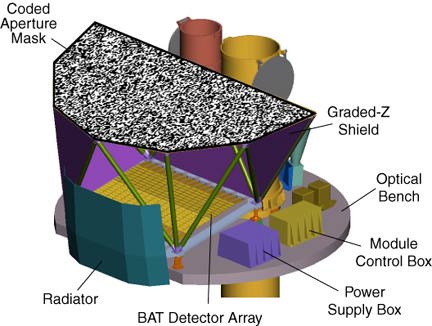
\includegraphics[width = \textwidth]{pictures/BAT.jpg}
			\caption{}
			\label{img:bat1}
		\end{subfigure}
		\begin{subfigure}[b]{0.40\linewidth}
		\centering
			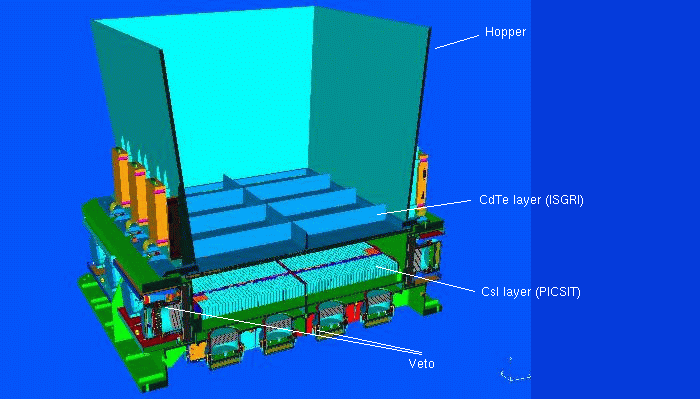
\includegraphics[width = \textwidth]{pictures/INTEGRAL.png}
			\caption{}
			\label{img:int1}
		\end{subfigure}
		\caption{Устройство прибора (a) BAT и (b) IBIS, частью которого является ISGRI}
	\end{figure}
	
	INTEGRAL аналогичен BAT, но его инструмент ISGRI использует CdTe-детекторы и его поле зрения равно $0.26$ стерадиан. На рис. \ref{img:int1} представлено его схематическое строение. 